\def\QRCODE{MASTER_mispa_TUT.IMG.image_segmentation_watershed_matlabqrcode.png}
\def\QRPAGE{http://www.iptutorials.science/tree/master/MASTER_mispa/TUT.IMG.image_segmentation_watershed/matlab}
\mcorrectionsection{Matlab correction}

\subsection{Watershed and distance map}
This method is a classical way of performing the separation of some objects by proximity or influence zones. It is illustrated in Fig.\ref{fig:watershed:matlab:dm}.

\begin{matlab}
A=imread('circles.tif');
% distance map
dist=bwdist(~A);
% watershed
watf=watershed(imcomplement(dist));
watf=(watf==0);
% separation of the grains
B=A & ~watf;
\end{matlab}

\begin{figure}[htbp]
 \centering
 \subfloat[Original image.]{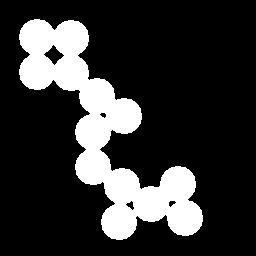
\includegraphics[width=.3\linewidth]{circles.jpg}}\hfill
 \subfloat[Distance map.]{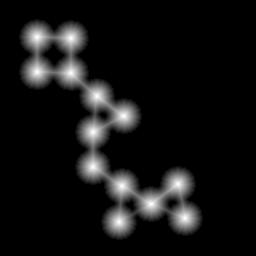
\includegraphics[width=.3\linewidth]{dist.jpg}}\hfill
 \subfloat[Separation of the grains.]{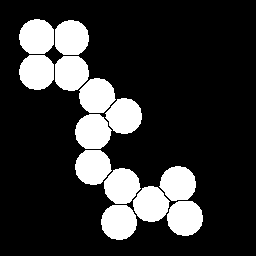
\includegraphics[width=.3\linewidth]{B.png}}
 \caption{Steps of the separation of the grains.}
 \label{fig:watershed:matlab:dm}
\end{figure}

\subsection{Watershed and image gradients}
The gradient image amplifies the noise. Thus, the watershed operator directly applied to the gradient of the image produces an over-segmented image (see Fig.\ref{fig:watershed:matlab:dm}).

\begin{matlab}
% read grayscale image
A=imread('gel.jpg');
% gradient
gradient=sobel(A);
rm=imregionalmin(gradient);
% watershed
wat=watershed(gradient);
wat=(wat==0);
\end{matlab}

\begin{figure}[htbp]
 \centering
 \subfloat[Original image.]{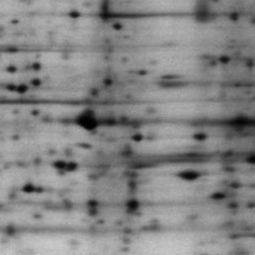
\includegraphics[width=.3\linewidth]{gel.jpg}}\hfill
 \subfloat[Amplitude of the gradient (Sobel).]{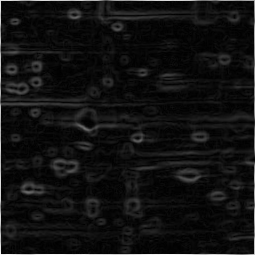
\includegraphics[width=.3\linewidth]{gradient.png}}\hfill
 \subfloat[Watershed segmentation.]{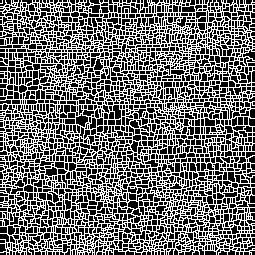
\includegraphics[width=.3\linewidth]{wat.jpg}}
 \caption{Performing the watershed on the gradient image is not a good idea.}
 \label{fig:watershed:matlab:wat}
\end{figure}

In fact, this method produces as many segments as there are minima in the gradient image Fig.\ref{fig:watershed:matlab:minima}.
\begin{figure}[htbp]
\centering
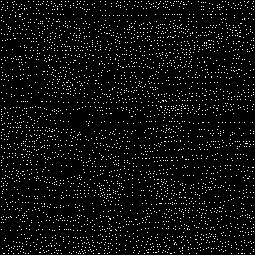
\includegraphics[width=.3\linewidth]{minima_gradient.png}
\caption{Local minima of the gradient image.}
 \label{fig:watershed:matlab:minima}
\end{figure}

\subsubsection{Solution: filtering the image}
Before evaluating the gradient, the image is filtered. The number of minima is lower and this leads to a less over-segmented image (Fig.\ref{fig:watershed:matlab:wat_filtered}).
\begin{matlab}
A=imread('gel.jpg');
% filtering
se = strel('disk',2);
AA=imopen(A,se);
f=imclose(AA,se);
% gradient
gradient=imgradient(f);
rm=imregionalmin(gradient);
% watershed
wat=watershed(gradient);
wat=(wat==0);
\end{matlab}

\begin{figure}[htbp]
 \centering
 \subfloat[Minima of the gradient after filtering the image.]{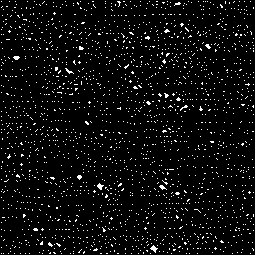
\includegraphics[width=.3\linewidth]{minima_filtered.png}}\hspace{1cm}
 \subfloat[Watershed segmentation.]{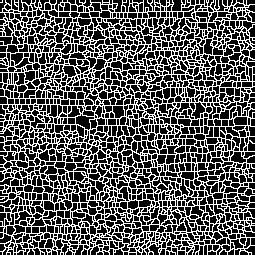
\includegraphics[width=.3\linewidth]{wat_filtered.jpg}}
 \caption{Even if the gradient is performed on the filtered image, there is still a high over-segmentation.}
 \label{fig:watershed:matlab:wat_filtered}
\end{figure}

\subsection{Watershed constrained by markers}
The watershed can be constrained by markers: the markers can provide the correct number of regions. This method imposes both the background
(external markers) and the objects (internal markers). The results are illustrated in Fig.\ref{fig:watershed:matlab:constrained}.
The ultimate erosion of the internal markers is used to deconnect these markers from the external markers.

\begin{matlab}
% filtering
se = strel('disk',2);
AA=imopen(A,se);
f=imclose(AA,se);
% internal markers (of the objects)
rm=imregionalmin(f);
rm = bwulterode(rm);
% external markers: watershed of filtered image
% background of the objects
watf=watershed(f);
watf=(watf==0);

% contrain the minima
gradient=imgradient(f);
mie=imimposemin(gradient, rm | watf);
minima=max(rm,watf);
% watershed constraint
watc=watershed(mie);
watc=(watc==0);
\end{matlab}

\begin{figure}[htbp]
 \centering
 \subfloat[Internal markers (blobs).]{
\includegraphics[width=.3\linewidth]{int_markers.png}} \hfill
 \subfloat[External (back\-ground) mar\-kers .]{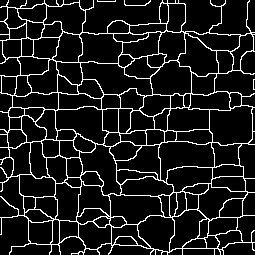
\includegraphics[width=.3\linewidth]{ext_markers.png}} \hfill
 \subfloat[Final seg\-men\-ta\-tion.]{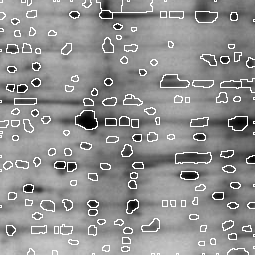
\includegraphics[width=.3\linewidth]{segmentation.png}}
 \caption{Watershed segmentation by markers.}
 \label{fig:watershed:matlab:constrained}
\end{figure}
